\section{Auswertung}

\subsection{Näherung des Films mit Hilfe des drei Temperatur Modell}
Die Messwerte für den Film werden mit Hilfe des drei Temperatur Modells

\begin{equation}
f(x) = A\exp{(Bx)} + C\exp{(Dx)} + E\exp{(Fx)}
\end{equation}

\noindent genähert um anschließend den Anteil des Films aus den weiteres Messungen abziehen zu können.

\begin{figure}[!htbp]
 	\centering
 	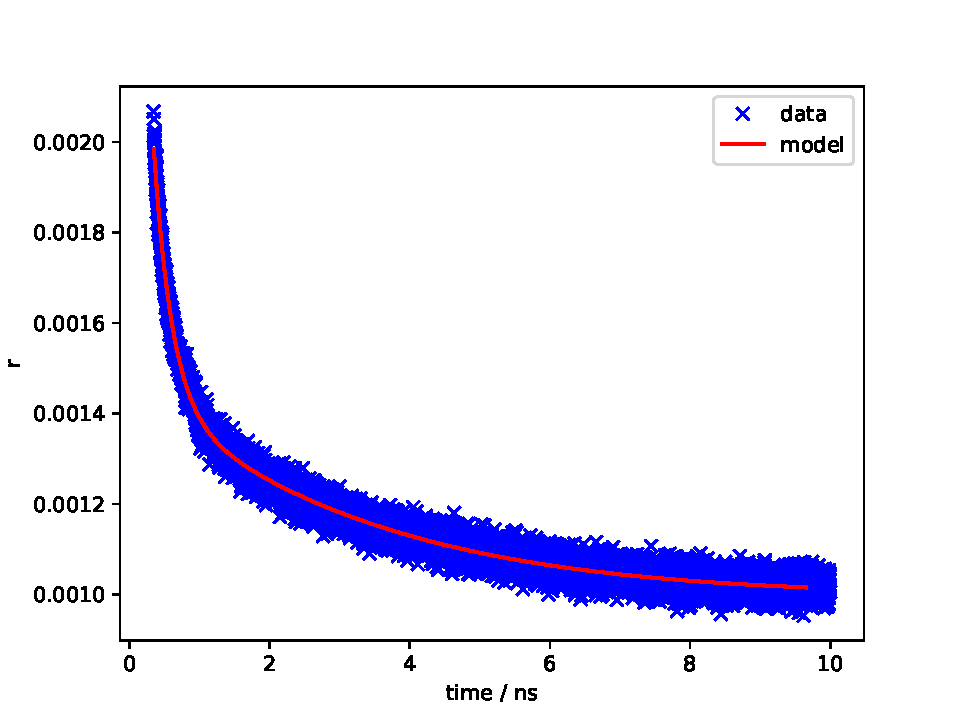
\includegraphics[width=\textwidth]{img/002_a000_b0_e245_FILM.pdf}
 	\caption{Messwerte für den gemesenen Film und die zugehörige Ausgleichsrechnung mit Hilfe des drei Temperatur Modells}
 	\label{abb:film}
\end{figure}

Die Ergebnisse der Ausgleichsrechnung sind in \autoref{abb:film} dargestellt. Die zugehörigen Koeffizienten finden sich in \autoref{tab:fit}.

\begin{table}[!htbp]
 \centering
\begin{tabular}{cc}
    Koeffizient & Wert \\
	\midrule
 	A & 0.00216 $\pm$ 0.00004 \\
 	B & -3.84 $\pm$ 0.05 \\
 	C & 0.00051 $\pm$ 0.00001 \\
 	D & -0.29 $\pm$ 0.01 \\
 	E & 0.00096 $\pm$ 0.00002 \\
 	F & 0.003 $\pm$ 0.001 \\
\end{tabular}
\caption{Ergenbisse der Ausgleichrechnung mit Hilfe des drei Temperatur Modells}
\label{tab:fit}
\end{table}

\newpage

\subsection{Korrektur der Daten}
Anschließend wird das Ergebniss der Ausgleichrechnung von den Messwerten der Messungen mit Gitter abgezogen.
In den Folgenden Abbildungen wurde lediglich ein kleiner Teil der Daten gezeichnet um die in den Messdaten enthaltenen 
Oszillationen sichtbar zu machen.

\begin{figure}[!htbp]
 	\centering
 	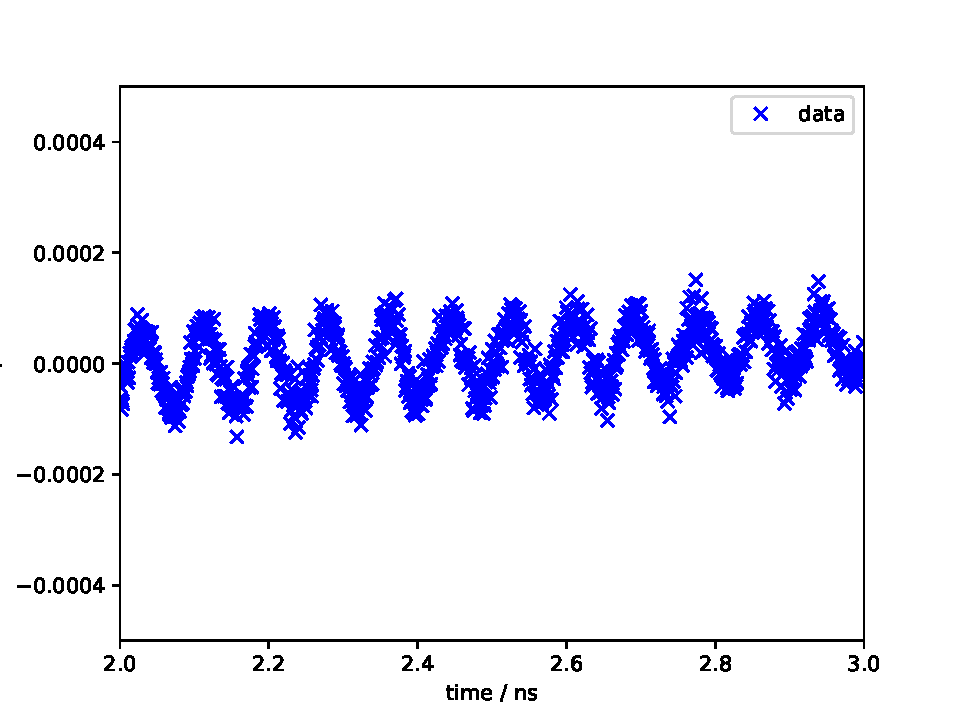
\includegraphics[width=\textwidth]{img/005_a000_b0_e245_G4corr.pdf}
 	\caption{Oszillationen in dem 23 nm tiefen Gitter}
 	\label{abb:film}
\end{figure}

\begin{figure}[!htbp]
 	\centering
 	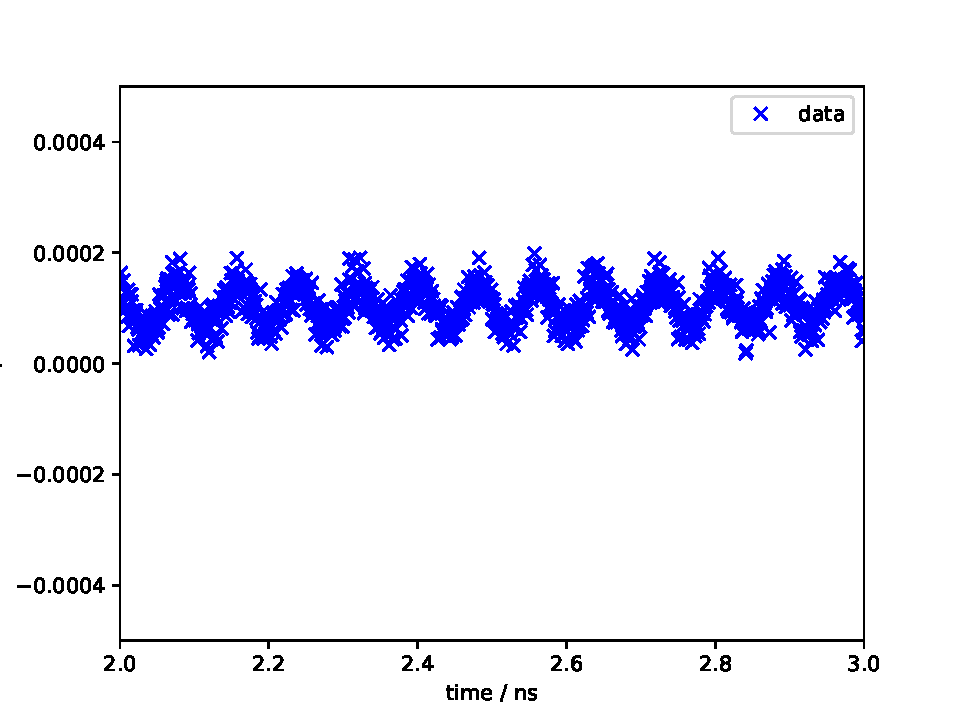
\includegraphics[width=\textwidth]{img/006_a000_b0_e245_G3corr.pdf}
 	\caption{Oszillationen in dem 17 nm tiefen Gitter}
 	\label{abb:film}
\end{figure}

\begin{figure}[!htbp]
 	\centering
 	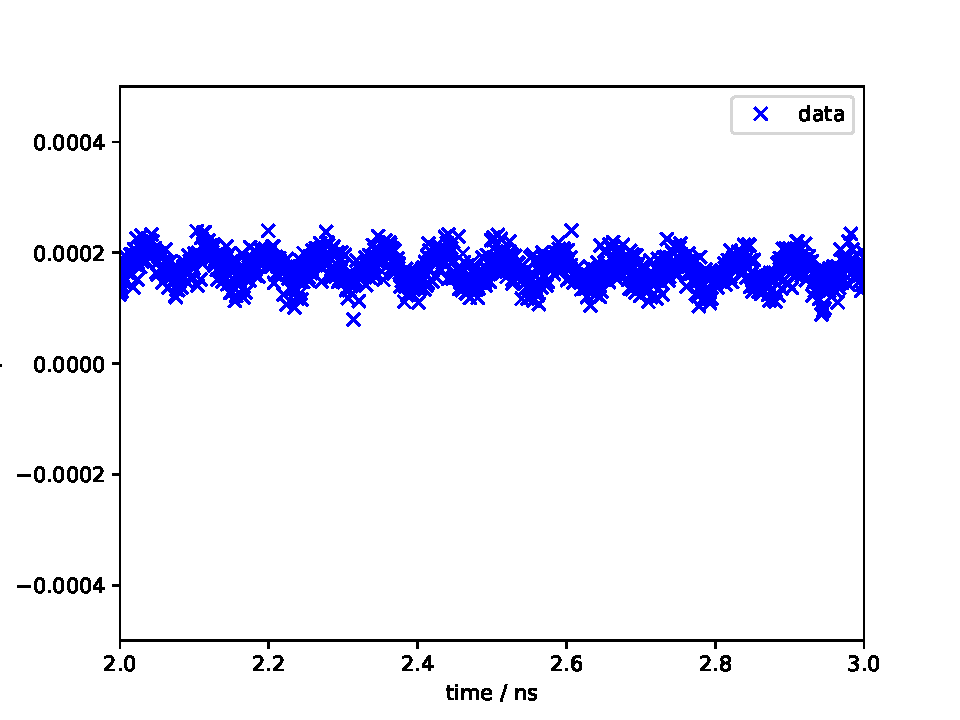
\includegraphics[width=\textwidth]{img/007_a000_b0_e245_G2corr.pdf}
 	\caption{Oszillationen in dem 14 nm tiefen Gitter}
 	\label{abb:film}
\end{figure}

\begin{figure}[!htbp]
 	\centering
 	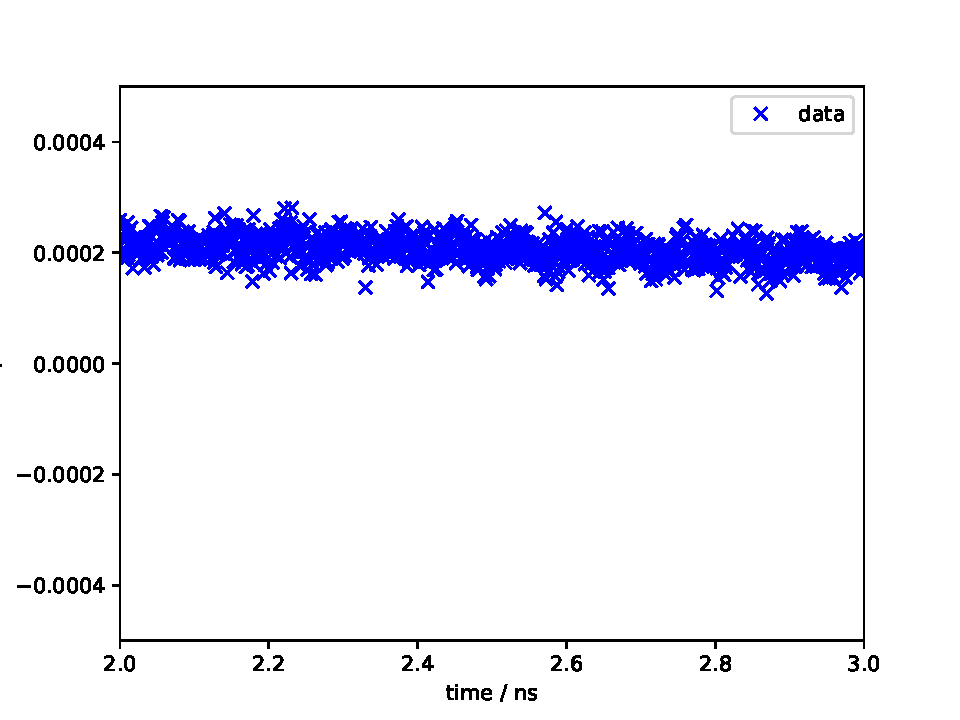
\includegraphics[width=\textwidth]{img/008_a000_b0_e245_G1corr.pdf}
 	\caption{Oszillationen in dem 7 nm tiefen Gitter}
 	\label{abb:film}
\end{figure}

\newpage

\subsection{Frequenzsprektren}
Die erhaltenen Oszillationen aus den Messdaten werden als periodisches Phänomen aufgefasst und mit Hilfe von Fouriermethoden analysiert. Es fällt auf, dass alle Frequenzspektren einen Peak bei ungefähr 12,2 GHZ aufweisen. Diese Frequenz ist charakteristisch für die benutzen Gitterbreiten und soll im folgenden genauer untersucht werden. An die Peaks wird ein Lorenzprofil der Form

\begin{equation}
L(\omega, \omega_0, \gamma) = \frac{1}{((\omega^2 - \omega_0^2)^2 + \gamma^2  \omega_02)}
\end{equation}

gefittet und im Anschluss die Halbwertsbreite und die Amplitude der enthaltenden Frequenz errechnen zu können. Es ist an dieser Stelle anzumerken, dass die Halbwertsbreite des Lorenzprofiles sich in guter Näherung zu $\gamma$ ergibt, da der Quotient aus $\gamma$ / $\omega_0$ << 1 ist.

\begin{figure}[!htbp]
 	\centering
 	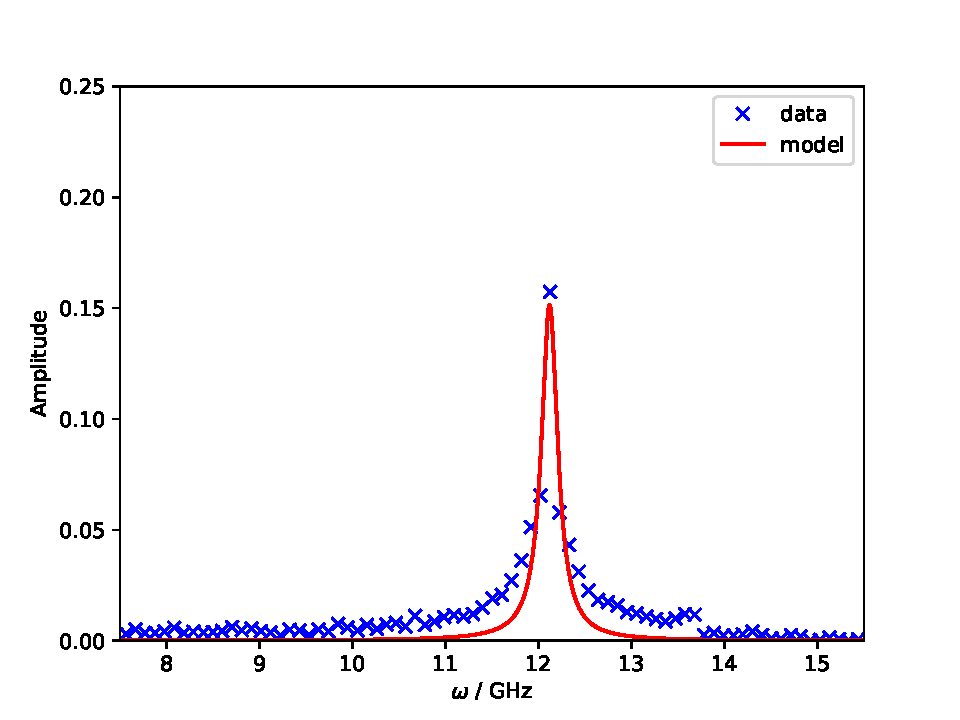
\includegraphics[width=\textwidth]{img/005_a000_b0_e245_G4fft.pdf}
 	\caption{Frequenzsprektrum für das 23\,nm tiefen Gitter}
 	\label{abb:film}
\end{figure}

\begin{table}[!htbp]
 \centering
\begin{tabular}{cc}
    Koeffizient & Wert \\
	\midrule
 	$\omega_0$ & 12,119 $\pm$ 0,006 \\
 	$\gamma$ & 0,212 $\pm$ 0,004 \\
\end{tabular}
\caption{Fit Ergebnisse für das Gitter mit 23\,nm tiefe}
\label{tab:fit}
\end{table}


\begin{figure}[!htbp]
 	\centering
 	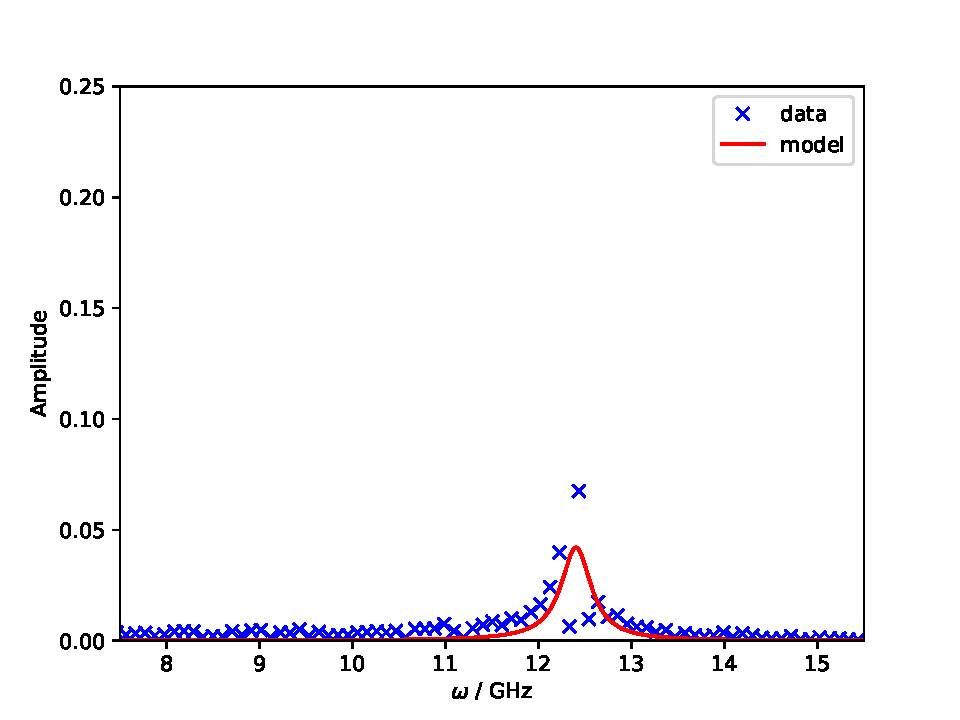
\includegraphics[width=\textwidth]{img/006_a000_b0_e245_G3fft.pdf}
 	\caption{Frequenzsprektrum für das 17\,nm tiefen Gitter}
 	\label{abb:film}
\end{figure}

\begin{table}[!htbp]
 \centering
\begin{tabular}{cc}
    Koeffizient & Wert \\
	\midrule
 	$\omega_0$ & 12,40 $\pm$ 0,03 \\
 	$\gamma$ & 0,39 $\pm$ 0.03 \\
\end{tabular}
\caption{Fit Ergebnisse für das Gitter mit 17\,nm tiefe}
\label{tab:fit}
\end{table}

\begin{figure}[!htbp]
 	\centering
 	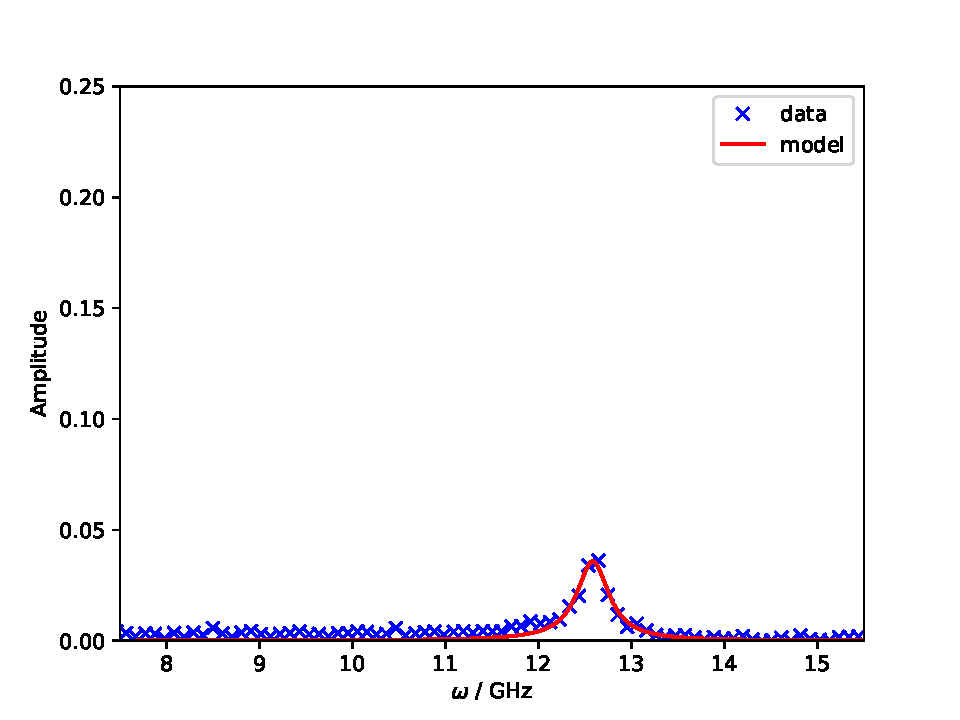
\includegraphics[width=\textwidth]{img/007_a000_b0_e245_G2fft.pdf}
 	\caption{Frequenzsprektrum für das 14\,nm tiefen Gitter}
 	\label{abb:film}
\end{figure}

\begin{table}[!htbp]
 \centering
\begin{tabular}{cc}
    Koeffizient & Wert \\
	\midrule
 	$\omega_0$ & 12,58 $\pm$ 0.05 \\
 	$\gamma$ & 0,42 $\pm$ 0,04 \\
\end{tabular}
\caption{Fit Ergebnisse für das Gitter mit 14\,nm tiefe}
\label{tab:fit}
\end{table}

\begin{figure}[!htbp]
 	\centering
 	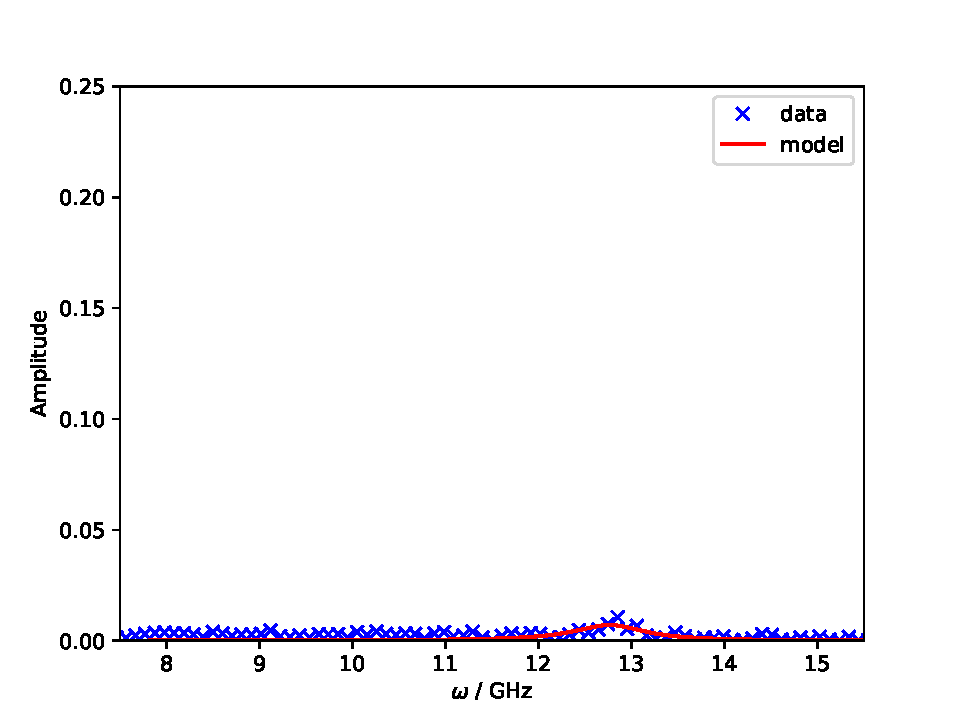
\includegraphics[width=\textwidth]{img/008_a000_b0_e245_G1fft.pdf}
 	\caption{Frequenzsprektrum für das 7\,nm tiefen Gitter}
 	\label{abb:film}
\end{figure}

\begin{table}[!htbp]
 \centering
\begin{tabular}{cc}
    Koeffizient & Wert \\
	\midrule
 	$\omega_0$ & 12,8 $\pm$ 0,4 \\
 	$\gamma$ & 0,9 $\pm$ 0,4 \\
\end{tabular}
\caption{Fit Ergebnisse für das Gitter mit 7\,nm tiefe}
\label{tab:fit}
\end{table}

\newpage

Im Anschluss werden die Amplituden der Frequenzkomponenten gegen die Tiefe des Gitters aufgetragen und eine Ausgleichsrechnung
mit einer linearen Funktion

\begin{equation}
f(x) = Ax + B
\end{equation}

\noindent durchgeführt.

\noindent Die Maximas der entsprechenden Frequenzkomponente ergibt sich mit aus dem höchsten Punkt des Lorenzprofiles. Dieser Punkt wird mit Hilfe einer
softwareseitigen peak detection bestimmt.

\begin{figure}[!htbp]
 	\centering
 	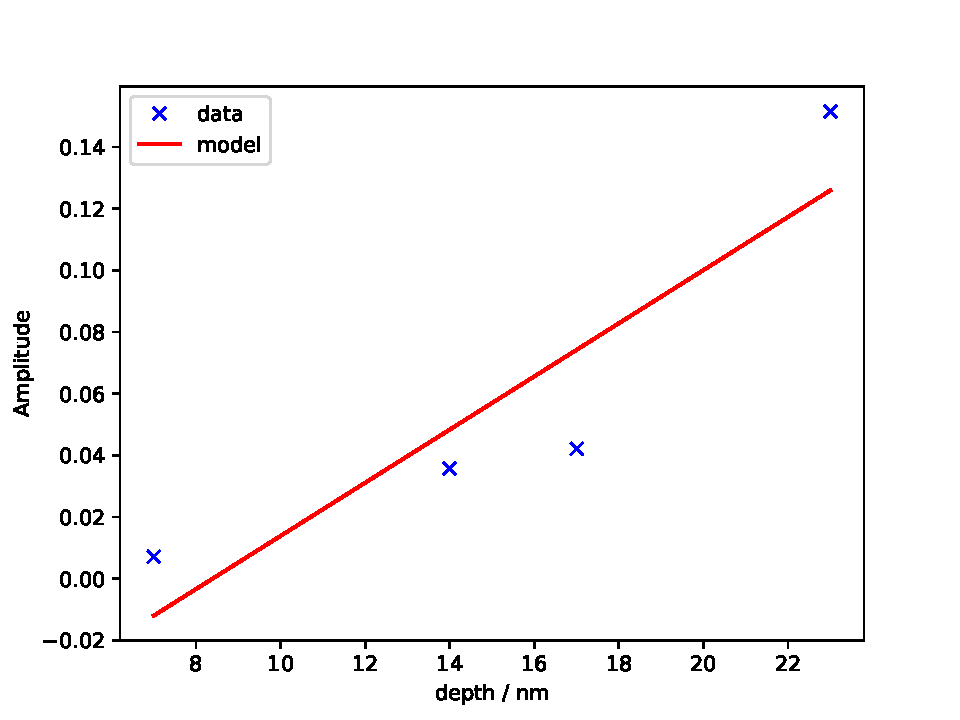
\includegraphics[width=\textwidth]{img/amplitudes.pdf}
 	\caption{Amplituden der charakteristischen Frequenzkomponente aufgetragen gegen die Gittertiefe und linearer Ausgleichsrechnung}
 	\label{abb:film}
\end{figure}

\begin{table}[!htbp]
 \centering
\begin{tabular}{cc}
    Koeffizient & Wert \\
	\midrule
 	A & 0.009 $\pm$ 0,003 \\
 	B & -0.07 $\pm$ 0,05 \\
\end{tabular}
\caption{Fit Ergebnisse für die Amplituden der verschiedenen Gitter in Abhängigkeit zur Gittertiefe}
\label{tab:fit}
\end{table}

\newpage

\subsection{Einfluss der Polarisation auf die Schwingung}

\begin{figure}[!htbp]
 	\centering
 	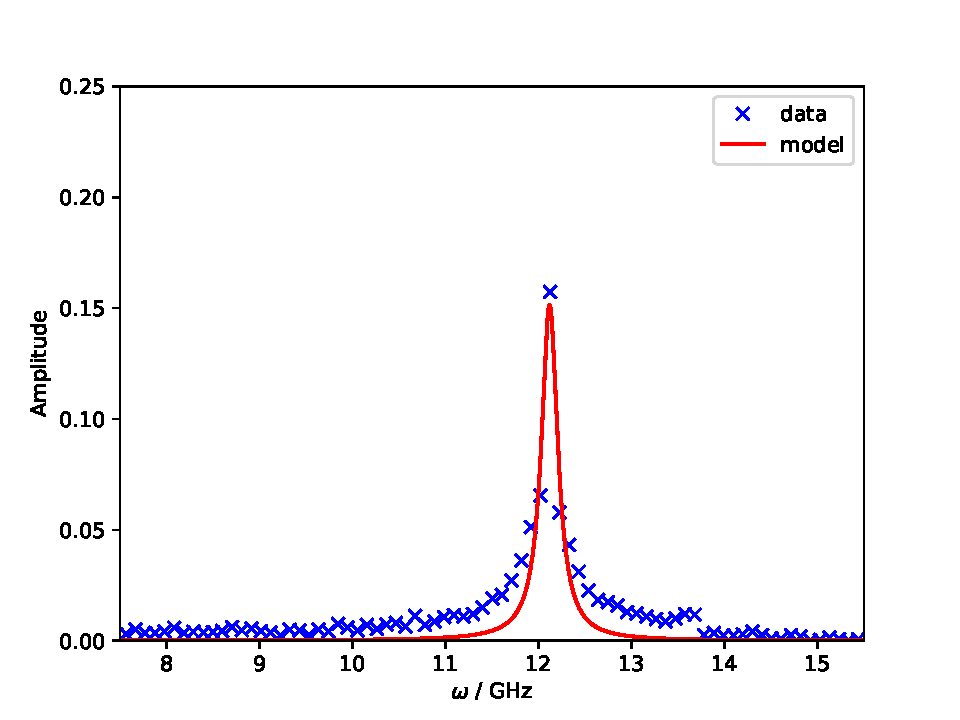
\includegraphics[width=\textwidth]{img/005_a000_b0_e245_G4fft.pdf}
 	\caption{Frequenzsprektrum für das 14\,nm tiefen Gitter unter einem Polarisationwinkel von 0 Grad}
 	\label{abb:film}
\end{figure}

\begin{table}[!htbp]
 \centering
\begin{tabular}{cc}
    Koeffizient & Wert \\
	\midrule
 	$\omega_0$ & 12,12 $\pm$ 0,01 \\
 	$\gamma$ & 0,211 $\pm$ 0,008 \\
\end{tabular}
\caption{Fit Ergebnisse für das Gitter mit 23\,nm tiefe unter einem Polarisationswinkel von 0 Grad}
\label{tab:fit}
\end{table}

\begin{figure}[!htbp]
 	\centering
 	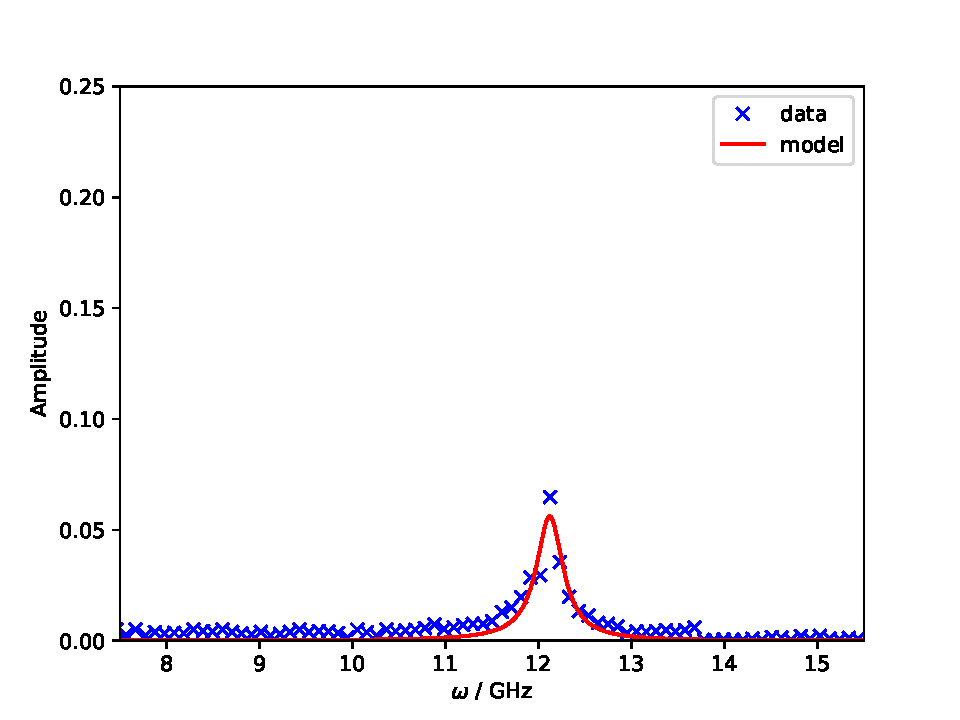
\includegraphics[width=\textwidth]{img/011_a000_b0_e245_G4_45fft.pdf}
 	\caption{Frequenzsprektrum für das 23\,nm tiefen Gitter unter einem Polarisationswinkel von 45 Grad}
 	\label{abb:film}
\end{figure}

\begin{table}[!htbp]
 \centering
\begin{tabular}{cc}
    Koeffizient & Wert \\
	\midrule
 	$\omega_0$ & 12,12 $\pm$ 0,01 \\
 	$\gamma$ & 0,36 $\pm$ 0,02 \\
\end{tabular}
\caption{Fit Ergebnisse für das Gitter mit 23\,nm tiefe unter einem Polarisationswinkel von 45 Grad}
\label{tab:fit}
\end{table}

\begin{figure}[!htbp]
 	\centering
 	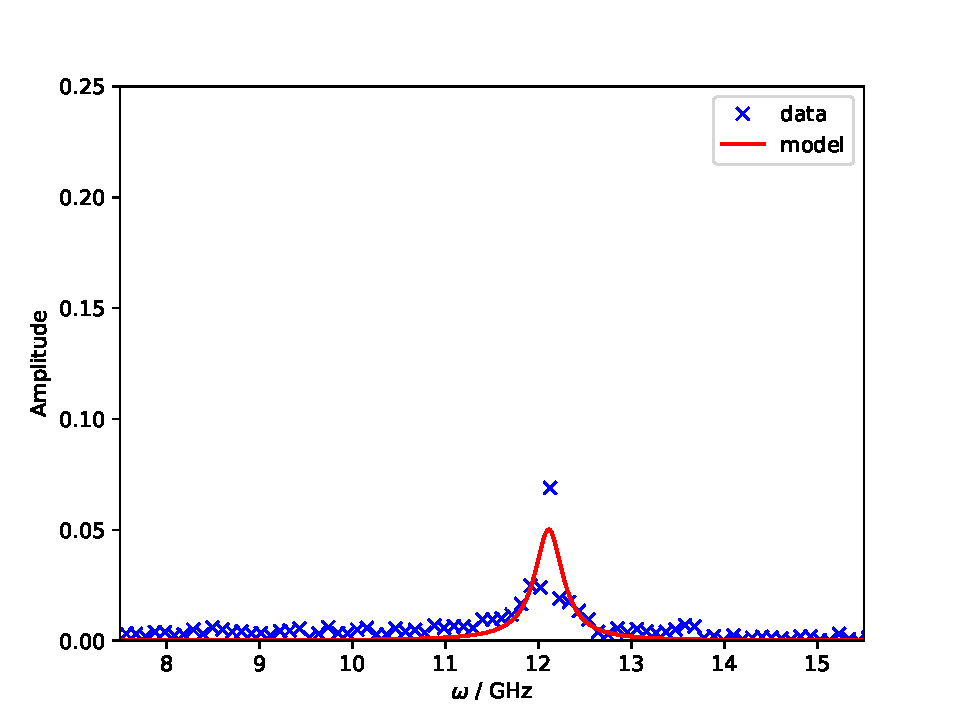
\includegraphics[width=\textwidth]{img/009_a000_b0_e245_G4_90fft.pdf}
 	\caption{Frequenzsprektrum für das 23\,nm tiefen Gitter unter einem Polarisationswinkel von 90 Grad}
 	\label{abb:film}
\end{figure}

\begin{table}[!htbp]
 \centering
\begin{tabular}{cc}
    Koeffizient & Wert \\
	\midrule
 	$\omega_0$ & 12,13 $\pm$ 0,02 \\
 	$\gamma$ & 0,34 $\pm$ 0,02 \\
\end{tabular}
\caption{Fit Ergebnisse für das Gitter mit 23\,nm tiefe unter einem Polarisationswinkel von 90 Grad}
\label{tab:fit}
\end{table}

\newpage
\subsection{Verbesserung der Signalqualität mit Hilfe eines Tiefpasses}
\noindent Abschließend soll noch der Einfluss eines Tiefpass Filters auf die Signalqualität überprüft werden. Dazu wird dass um das drei Temperatur Modell korrigierte Signal mittels FFT in den Frequenzraum transformiert und anschließend alle Frequenzanteile größer 16$\,$GHz auf 0 gesetzt.
Das resultierende Spektrum wird wieder zurücktransformiert und die Signale verglichen. Es ist anzumerken, das  

\begin{figure}[!htbp]
 	\centering
 	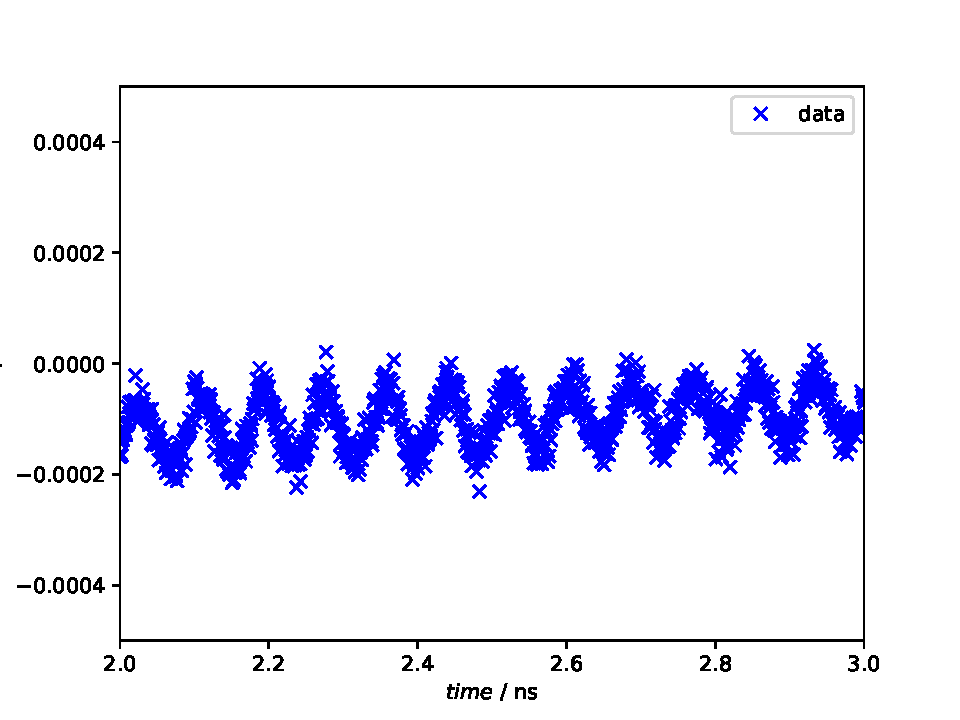
\includegraphics[width=\textwidth]{img/003_a000_b0_e245_G4corr.pdf}
 	\caption{Korrigiertes Signal für 20.000 Messwerte pro Datenpunkt}
 	\label{abb:film}
\end{figure}

\begin{figure}[!htbp]
 	\centering
 	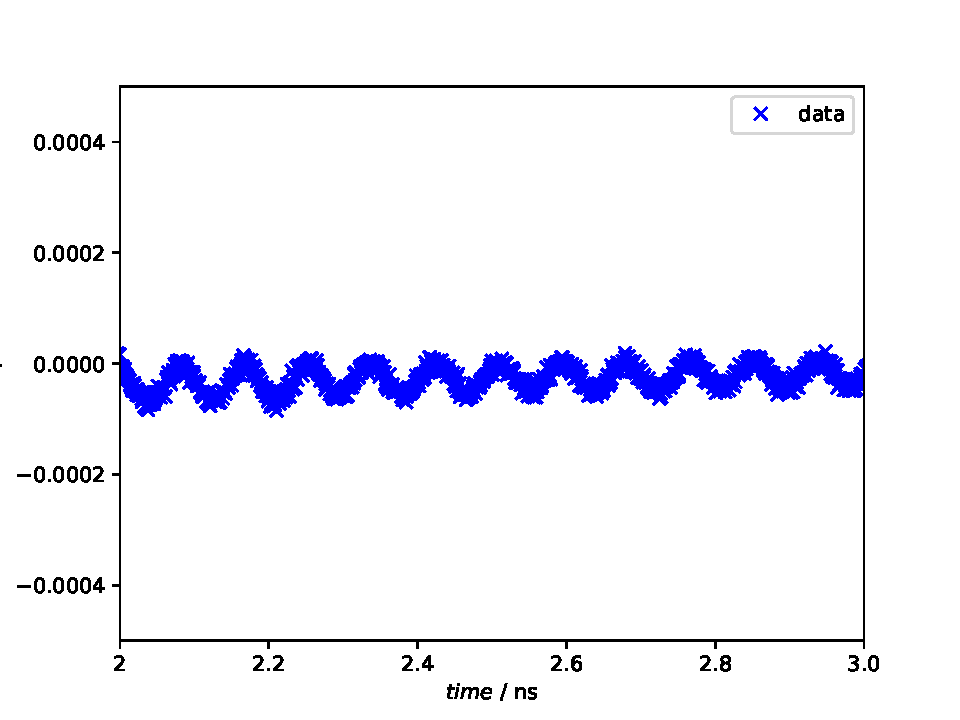
\includegraphics[width=\textwidth]{img/003_a000_b0_e245_G4lowpass.pdf}
 	\caption{Korrigiertes Signal für 20.000 Messwerte pro Datenpunkt nach dem Tiefpass}
 	\label{abb:film}
\end{figure}

\begin{figure}[!htbp]
 	\centering
 	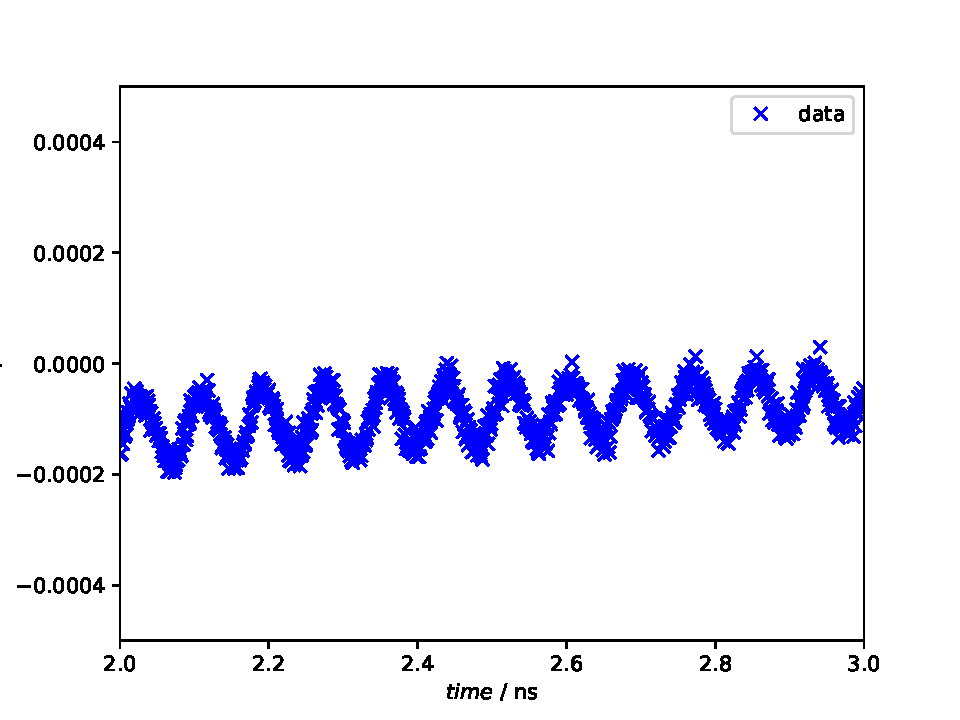
\includegraphics[width=\textwidth]{img/004_a000_b0_e245_G4corr.pdf}
 	\caption{Korrigiertes Signal für 50.000 Messwerte pro Datenpunkt}
 	\label{abb:film}
\end{figure}

\begin{figure}[!htbp]
 	\centering
 	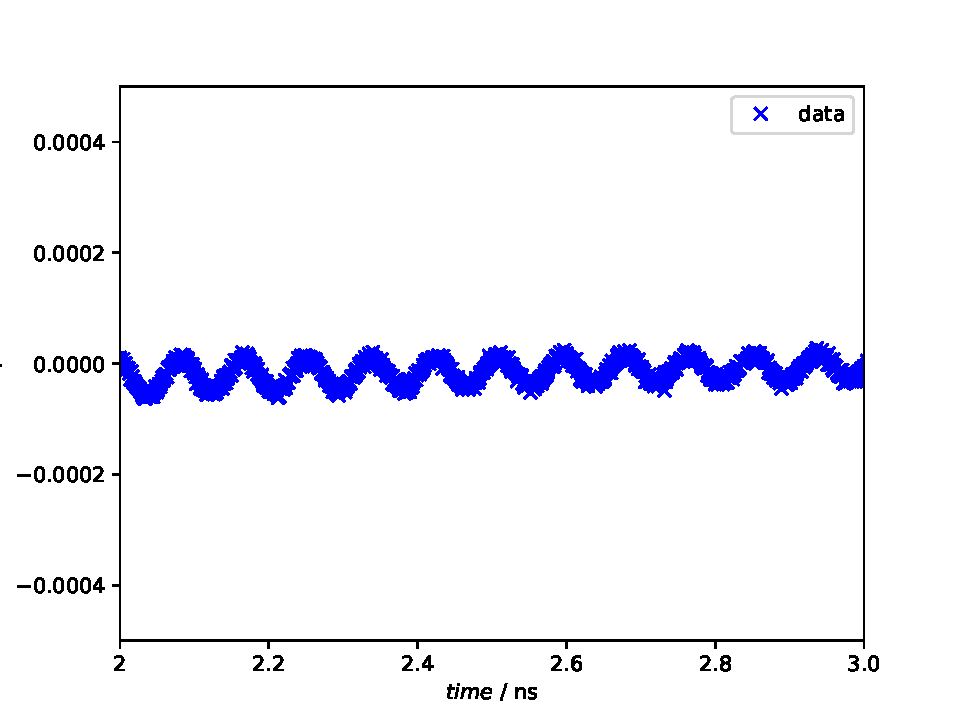
\includegraphics[width=\textwidth]{img/004_a000_b0_e245_G4lowpass.pdf}
 	\caption{Korrigiertes Signal für 50.000 Messwerte pro Datenpunkt nach dem Tiefpass}
 	\label{abb:film}
\end{figure}

\newpage